\section*{Part 1}
\subsection*{1.1}
\subsubsection*{Variables, domains, and constrains}
For the letter-based assignment version of backtracking search, the variables are each position in the result array. The domain for each position in the set contains all letters that appear in the candidate word lists for each of the categories that the position must satisfy. For example, if the puzzle contains the lines
\begin{verbatim}
emotion: 4, 5, 7
adverb: 1, 5, 9
interjection: 4, 5, 6
\end{verbatim}
then the variable for position 5 has the domain that contains all letters that appear in the emotion, adverb, and interjection lists. The constraint on the letter values of the positions is that each position must take on a letter value that is in all of the candidate lists that the position must satisfy. Using the above example, position 5 cannot have the letter ``Z'' since it does not appear in any word in the emotion and adverb word lists. Also, the three variables that must satisfy forming a word in their given category must together have the letter values that make up one of the words in that category.

For the word-based assignment version, the variables are the sets of three positions whose letters must be a word from their designated category's list. The domains of one of these variables contains the 3! permutations of each of the three-letter words in the word list of their designated category. These variables are constrained such that the three positions must together have letter values that make up one of the words in their category's word list.
\subsubsection*{Design and implementation}
We design the puzzle data structure as an array of tuples which contains neccessary information for checking: the required categories for each slot, the corresponding position of this slot at the category. In order to optimize the efficiency of our searching, we choose the most constraining variable to assign first.
For letter based search, for each slot we keep a set of viable letter candidates that can fit in. The set of candidates is initially acquired by the union of the letter at corresponding position of categories that are required to fill in this slot. As we assign values and do the searching further, we will keep removing the invalid candidates in the set by arc consistency.
For word based search, we choose the category with the least candidates to choose from. For each category we have a set of feasible candidates for it, which are initially built from the wordset. When assigning the value of each candidates, we will check the categories who share the same slots with the current candidates and remove the invalid candidates introduced by this assignment by arc consistency, and propagate the pruning to all the slots that will be affected.
\subsubsection*{Solutions and search traces}
The solutions are consistent between letter-based search and word-based search.\\
Note: as we do not sequentially assign letters to each slot, instead we pick the slot with less candidates to improve our efficiency, we cannot show our path as sequential as in the example trace. For example, for tuple (4, 'A'), it means it tris to fill slot 5 (the index starts from 0) with letter A.
\paragraph{Puzzle 1}
Solutions:\\
\begin{verbatim}
[['N', 'N', 'E', 'M', 'A', 'N', 'D', 'Y', 'E'],
  ['N', 'W', 'E', 'M', 'A', 'N', 'D', 'Y', 'E'],
  ['N', 'N', 'E', 'S', 'A', 'Y', 'D', 'Y', 'E'],
  ['N', 'W', 'E', 'S', 'A', 'Y', 'D', 'Y', 'E']]
Search trace:
Letter based:
(4, 'A'),
(6, 'D'),
(0, 'N'),
(8, 'E'),
(3, 'M'),
(2, 'E'),
(5, 'N'),
(7, 'Y'),
(1, 'N'), => NNEMANDYE
(1, 'W'), => NWEMANDYE
(3, 'S'),
(2, 'E'),
(5, 'Y'),
(7, 'Y'),
(1, 'N'), => NNESAYDYE
(1, 'W'), => NWESAYDYE
Word based:
search order: emotion -> body -> interjection -> adverb -> verb -> adjective
      root -> MAD     -> EYE  -> MAN          -> NAE    -> DYE  -> NEE       => NNEMANDYE
                                                                -> WEE       => NWEMANDYE
              SAD     -> EYE  -> SAY          -> NAE    -> DYE  -> NEE       => NNESAYDYE
                                                                -> WEE       => NWESAYDYE
\end{verbatim}
\paragraph{Puzzle 2}
Solutions:\\
\begin{verbatim}
[['H', 'S', 'I', 'A', 'I', 'W', 'N', 'C', 'S'],
['H', 'S', 'I', 'A', 'I', 'W', 'N', 'P', 'S'],
['H', 'S', 'I', 'O', 'I', 'W', 'N', 'D', 'S'],
['H', 'S', 'I', 'O', 'I', 'W', 'N', 'Y', 'S']]
Search trace:
Letter based:
(8, 'S'),
(1, 'S'),
(4, 'I'),
(6, 'N'),
(0, 'H'),
(2, 'I'),
(5, 'W'),
(3, 'A'),
(7, 'C'), => HSIAIWNCS
(7, 'P'), => HSIAIWNPS
(3, 'O'),
(7, 'D'), => HSIOIWNDS
(7, 'Y'), => HSIOIWNYS
Word based:
Search order: pronoun -> palindrom -> interjection -> math -> verb -> noun
root       -> HIS     -> SIS       -> HAW          -> SIN  -> SAW  -> SAC  => HSIAIWNCS
           -> HIS     -> SIS       -> HAW          -> SIN  -> SAW  -> SAP  => HSIAIWNPS
                                   -> HOW          -> SIN  -> SOW  -> SOD  => HSIOIWNDS
                                                                   -> SOY  => HSIOIWNYS
\end{verbatim}
\paragraph{Puzzle 3}
Solutions:\\
\begin{verbatim}
[['A', 'S', 'U', 'L', 'P', 'E', 'A'],
['A', 'S', 'U', 'L', 'P', 'I', 'E']]
Search trace:
Letter based:
(4, 'P'),
(5, 'E'),
(0, 'A'),
(1, 'S'),
(2, 'U'),
(3, 'L'),
(6, 'A'), => ASULPEA
(5, 'I'),
(0, 'A'),
(1, 'S'),
(2, 'U'),
(3, 'L'),
(6, 'E')  => ASULPIE
Word based:
Search order: nature -> food -> animal -> noun -> interjection
root       -> ALP    -> PEA  -> ASP    -> LEA  -> SUP          => ASULPEA
                     -> PIE  -> ASP    -> LIE  -> SUP          => ASULPIE
\end{verbatim}
\paragraph{Puzzle 4}
Solutions:\\
\begin{verbatim}
[['H', 'E', 'D', 'I', 'T', 'Y', 'R', 'E'],
['H', 'E', 'L', 'I', 'T', 'Y', 'R', 'E'],
['H', 'E', 'T', 'I', 'T', 'Y', 'R', 'E']]
Search trace:
Letter based:
(1, 'E'),
(0, 'H'),
(5, 'Y'),
(3, 'I'),
(4, 'T'),
(6, 'R'),
(7, 'E'),
(2, 'D'), => HEDITYRE
(2, 'L'), => HELITYRE
(2, 'T')  => HETITYRE
Word based:
Search order: body -> pronoun -> interjection -> computer -> noun -> verb
root       -> EYE  -> HER     -> HEY          -> HIT      -> IRE  -> DIE  => HEDITYRE
                                                                  -> LIE  => HELITYRE
                                                                  -> TIE  => HETITYRE
\end{verbatim}
\paragraph{Puzzle 5}
Solutions:\\
\begin{verbatim}
[['I', 'H', 'T', 'T', 'N', 'O', 'I', 'E', 'N'],
['I', 'H', 'T', 'T', 'Y', 'O', 'I', 'E', 'N'],
['T', 'H', 'T', 'T', 'N', 'O', 'I', 'E', 'N'],
['T', 'H', 'T', 'T', 'Y', 'O', 'I', 'E', 'N']]
Search trace:
Letter based:
(2, 'T'),
(3, 'T'),
(6, 'I'),
(5, 'O'),
(7, 'E'),
(8, 'N'),
(1, 'H'),
(0, 'I'),
(4, 'N'), => IHTTNOIEN
(4, 'Y'), => IHTTYOIEN
(0, 'T'),
(4, 'N'), => THTTNOIEN
(4, 'Y')  => THTTYOIEN
Word based:
Search order: number -> container -> music -> body -> animal -> adverb -> noun
root       -> TEN    -> TIN       -> TIE   -> TOE  -> HEN    -> NON    -> ION  => IHTTNOIEN
                                                                       -> TON  => THTTNOIEN
                                                             -> YON    -> ION  => IHTTYOIEN
                                                                       -> TON  => THTTYOIEN
\end{verbatim}
\subsection*{1.2}
\subsubsection*{Generating an intersection-free graph}
Our algorithm generates a graph by adding one node at a time and adding edges between it and all other possible nodes. For a new node $O$, we iterate through all the other nodes $C$ that are already in the graph and check if joining $O$ and $C$ with a segment would intersect any existing segment $\overline{AB}$. For each $C$, we iterate through an array tracking all segments we currently have between two nodes. We represent each segment using the equation
\begin{equation}
  f_{ab}(x,y) = \frac{y-y_a}{y_b-y_a} - \frac{x-x_a}{x_b-x_a}
\end{equation}
where $y_b \ne y_a$ and $x_b \ne x_a$ since either of these would result in a point rather than a segment.

If $O$ and $C$ are on the same side of $\overline{AB}$, then $f_{ab}(O)$ and $f_{ab}(C)$ would both be either positive or negative when the coordinates of $O$ and $C$, respectively, are substituted into $f_{ab}$. In this case, $O$ and $C$ can be joined since $\overline{OC}$ would not cross $\overline{AB}$.

If $f_{ab}(O)$ and $f_{ab}(C)$ have different signs, then it is possible that $\overline{OC}$ intersects $\overline{AB}$. Therefore, we must check if the largest angle between $\angle AOB$, $\angle COB$ and $\angle AOB$ is $\angle AOB$. If it is, then there will be an intersection. Otherwise, $\overline{OC}$ would pass above or below $\overline{AB}$, in which case a segment can be drawn between $O$ and $C$. Thus, we must check that $max(\angle AOB, \angle COB, \angle AOB)\ne \angle AOB$, or the equivalent $min(cos\angle AOB, cos\angle COB, cos\angle AOC) \ne cos\angle AOB)$.

Once we check that $\overline{OC}$ for some $C$ does not intersect any of the segments currently in the graph, we add $\overline{OC}$ to our segment list and continue checking for all other $C$ in the graph. We perform this process for every node $O$ that we add to the graph.

Larger N take much longer to generate the graph, so a sampling of N values is shown. Also note that the average number of assignments for (b) can be below N since some nodes were passively assigned colors by the removal of all other colors from their list via forward checking.

\begin{tabular}{r|l|l|l}
  N & average number of edges & average number of assignments (a) & average number of assignments (b) \\
  \hline
  5 & 8.0 & 5 & 5 \\
  10 & 20.4 & 10 & 9 \\
  20 & 50.6 & 209 & 15 \\
  %% 25 & 67.0 & & 18 \\
\end{tabular}

\begin{tabular}{r|l|l}
  N & average running time (a) & average running time (b) \\
  \hline
  5 & 0.000260829925537 & 0.00047965 \\
  10 & 0.000330924987793 & 0.000859022140503 \\
  20 & 0.00399613380432 & 0.001936007 \\
  %% 25 & & 0.00184202194214 \\
\end{tabular}

\subsubsection*{Subquestion a}
When we generated the graph, we kept a list of all nodes. Therefore, we can randomly select from this list the next node to assign a value to. The color value to assign is selected randomly from a list of four colors. If any constraints are violated, our algorithm backtracks, reassigns a value to a previous node and attempts to complete the assignment. It continues to backtrack and reassign until it achieves a satisfactory assignment. Below is an example where N=20.

\begin{figure}[H]
  \centering
  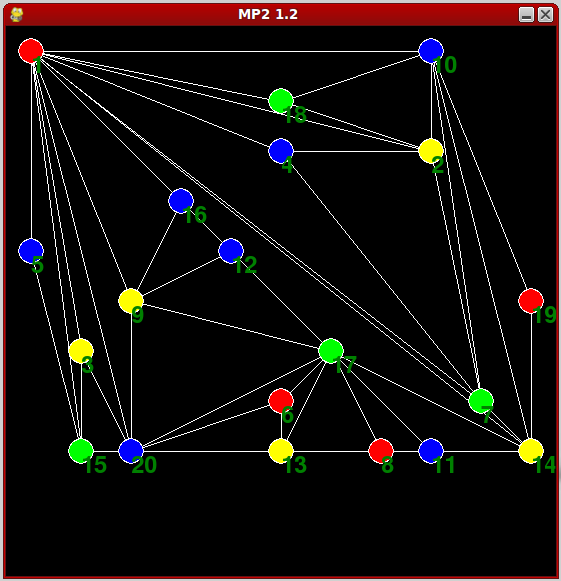
\includegraphics[width=0.3\textwidth]{graphics/rand_assign_20.png}
\end{figure}

\subsubsection*{Subquestion b}
Our forward checking algorithm eliminates colors from a node's list of possible colors as its neighbors colors are set. The algorithm selects the most constrained variable to assign a value to first, where the most constrained variable is the node with the fewest remaining colors. We select the color to assign by iterating through all possible colors remaining for the node, computing how many of its neighbors have that color and would need to have it removed from their remaining colors list, and assign to the node the color for which the fewest number of neighbors must have their list reduced. Below is an example where N=20.

\begin{figure}[H]
  \centering
  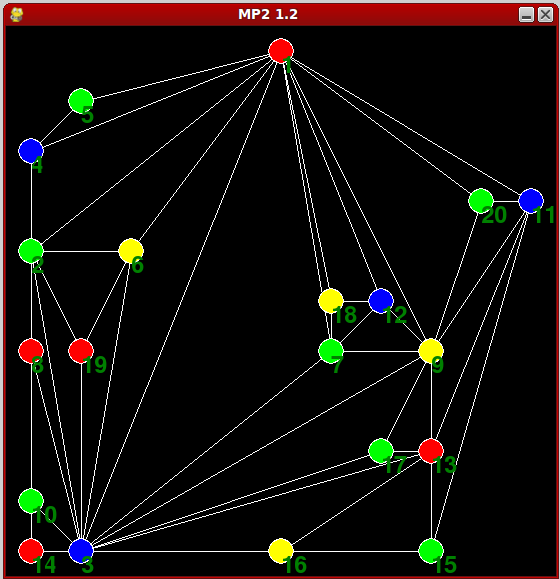
\includegraphics[width=0.3\textwidth]{graphics/forward_assign_20.png}
\end{figure}

\subsubsection*{Extra credit: local search}
Our local search algorithm first iterates through the list of nodes in the graph, and for each node, randomly selects a color from a color list to assign to it. Then, we start at the first node in the graph's node list and check if any of its neighbors share its color. If so, we reassign those neighbors to other colors and add them to a queue of nodes whose neighbors must be checked, if they hadn't been added in this iteration before. We continue dequeuing nodes and checking their neighbors until the queue is empty.

We then check if the assignment of colors is consistent, i.e. no neighbors share colors. If not, we initiate another round of reassignment as described above. We do this until the assignment of colors is consistent. Since a graph without intersections is equivalent to a map, by the four-color theorem, there must exist a four-color coloring of any graph we generate. Below is an example where N=10, followed by the data provided for previous parts of 1.2.

\begin{figure}[H]
  \centering
  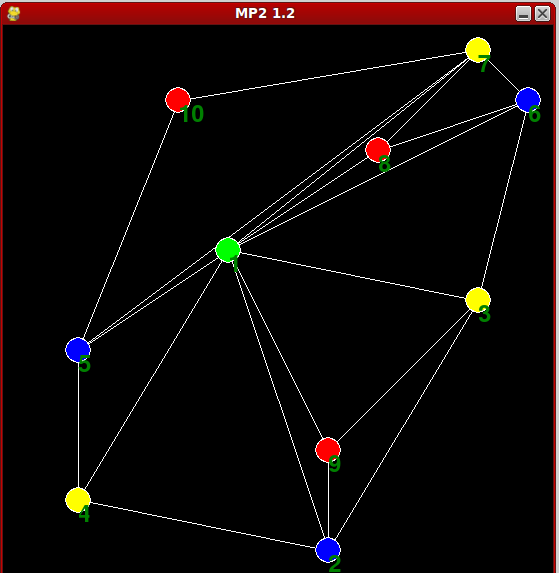
\includegraphics[width=0.3\textwidth]{graphics/local_assign_10.png}
\end{figure}

\begin{tabular}{r|l|l|l}
  N & edges & variable assignments & running time \\
  \hline
  5 & 8.0 & 7.2 & average number of edges \\
  10 & 20.6 & 23.8 & 0.000926971 \\
\end{tabular}